\documentclass[a4paper, 11pt]{article}
\usepackage[polish]{babel}
\usepackage[MeX]{polski}
\usepackage[utf8]{inputenc}
\usepackage[T1]{fontenc}
\usepackage{graphicx}
\usepackage{float}
\begin{document}
\renewcommand\refname{Bibliography}
\renewcommand{\figurename}{Figure}
	\begin{center}
			\begin{LARGE}
			Spread of epidemic\\[1cm]
		    \end{LARGE}
	    	\begin{Large}
	    		Author: Marcin Jędrzejczyk \\
	    		Supervisor: Dr hab. inż. Jarosław Wąs\\[1cm]
	    	\end{Large}
	\end{center}

	\section{Introduction}
	When disease spread quickly and affect many people we can call it epidemic. Some of the most unfamus epidemic thorough history are XIV century Black Death and Spanish  Flu pandemic in 1918. Infected person is not significant, however when a great number of people is sick it creates serious health and economic threats. Goal of simulating spread of epidemic is to better understand how epidemic behave in time, how quickly it spreads depending on many factors.\cite{WHITE} It can also be used to picture how vaccination affect disease spreading and confirms that herd immunity is important.
	\section{Literature models}
	Main models for epidemic in cellular automata are as follows:\\
	\begin{itemize}
		\item SIR
		\item SEIR
		\item SIS
		\item SEIRS	
	\end{itemize}
	where each letter stand for status types of persons:
	\begin{itemize}
		\item S - susceptible 
		\item I - infected 
		\item E - exposed
		\item R - recovered
	\end{itemize}
	The choosen model should represent a disease we want to model. SIR model assume that in recovery status individual get full immunity and on the other hand in SIS person can get sick even after successful treatment.\cite{WHITE}\\
	
	The neighborhood we choose can greatly affect dynamics of disease spreading as stated in \cite{cisse}. However more than type of neighborhood the type of connection between cells is important. There can be one, two three or none ways of transport. It affects equations and speed of spreading.\cite{WHITE} \\
	
	Each cell is not an individual person, but a representation of square portion of land. That said there can be a cell with only infected people in it. People can move from one cell to another.\cite{WHITE}  \\
	
	During next step model calculate how many people will be in each cell in each of groups(susceptible,infected,exposed,recovered). Vaccinations, cell connections, neighbourhood and people spread are major factors in how disease will spread.

\section{Project goals}

The aim of this project is to implement SIR model of epidemic spread in cellular automata with JAVA. Main programming reference will be code from laboratory classes where cellular automata was used. The UI will be created with JavaFX and SceneBuilder. If possible interface  will have may parameters to choose, like: vaccination value,  people spread in board(random,uniform, constant), epidemic model(SIR,SIS,SEIR,SEIRS), neighbourhood size and type, if not only simple parameters for one model will be present. 

\begin{figure}[H]
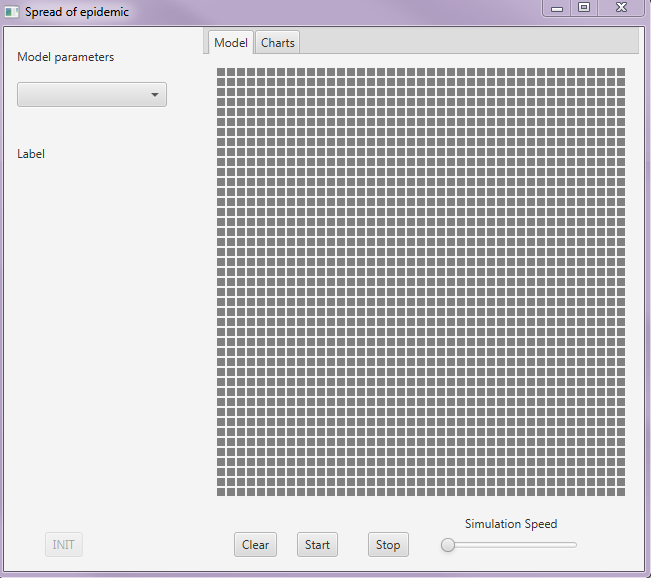
\includegraphics[scale=0.9]{GUI1.PNG} 
\caption{Prototype of user interface}
\end{figure}

	
	\bibliographystyle{plain}% plain/abbrv/alpha
	\bibliography{mybib}
	
\end{document}